%\documentclass[a4paper]{article}
%\usepackage[T1]{fontenc}
%\usepackage[utf8]{inputenc}
%\usepackage[italian]{babel}
%\usepackage{amsmath}
%\usepackage{hyperref}
%\usepackage{amsthm}
%\usepackage{graphicx}
\documentclass[journal, a4paper]{IEEEtran}
\usepackage[italian]{babel}
\usepackage{booktabs}
\usepackage{siunitx}%Questo serve a caricare il pacchetto delle unità di misura del sistema internazionale%
\usepackage[utf8]{inputenc}
\usepackage{graphicx} 
\usepackage{url}
\usepackage{amsmath}
\usepackage{amssymb}
\usepackage{caption}
\usepackage{ textcomp }

\usepackage{keyval}
\usepackage{xcolor}
\usepackage{tikz}
\usepackage{circuitikz}
\usepackage{authblk}
%\usepackage{hyperref}

\begin{document}


% Define document title and author
	\title{Tecnologie Digitali - Relazione: convertitore di impedenza negativa e circuito Howland}
	\author[1]{Salvatore Bottaro}
		\author[2]{Lorenzo M. Perrone}
		\affil[1]{\texttt{salvo.bottaro@hotmail.it}}
		\affil[2]{\texttt{lorenzo.perrone.lmp@gmail.com}}
	\markboth{Tecnologie Digitali - Di Lieto}{}
	\maketitle

\begin{abstract}
In questa relazione mostriamo le caratteristiche e i limiti di un convertitore di impedenza negativa e la sua applicazione nel circuito Howland.
\end{abstract}

\section{Convertitore di impedenza negativa}
Si consideri il circuito in figura \ref{fig:negimp}.

\begin{figure}[htp]
\centering
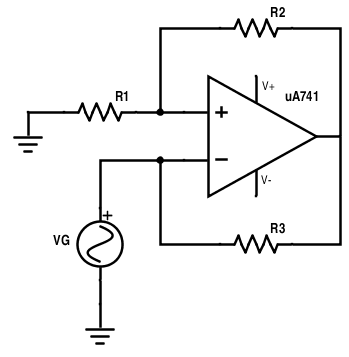
\includegraphics[scale=.5]{negative-impedance-converter}
\caption{Convertitore di impedenza negativa}
\label{fig:negimp}
\end{figure}

Si mostri in che senso esso sia un convertitore di impedenza negativa applicando le regole d'oro dell'op-amp e risolvendo le equazioni del circuito. Come si vede in figura \ref{fig:negimp} la tensione $V_{In+}$ all'ingresso non-invertente dell'op-amp è la tensione $V_g$ del generatore VG. Per le regole d'oro dell'op-amp si ha la stessa tensione all'ingresso invertente ed essendo l'op-amp in configurazione non-invertente, tale tensione viene amplificata di un fattore $1+\frac{R_2}{R_1}$, da cui:
\begin{equation}
V_{out} = (1+\frac{R_2}{R_1})V_{in}
\label{eqn:amp}
\end{equation}

Pertanto la corrente che scorre da $V_{In+}$ a $V_{out}$ è data da:
\begin{equation}
I = \frac{V_{In+} - V_{out}}{R_3} = -\frac{R_2}{R_1 \, R_3}\, V_g \, \rightarrow V_g = -\frac{R_1\,R_3}{R_3}\,I
\end{equation}
da cui si evince come il generatore "veda" un'impedenza equivalente negativa.\\
Poiché l'espressione della resistenza equivalente segue direttamente dall'equazione \ref{eqn:amp} si ha che un modo per verificare il corretto comportamento del circuito è verificare se l'op-amp si comporta correttamente in configurazione non-invertente e dunque cercare di delineare i limiti di tale configurazione.\\
Per quanto riguarda il dimensionamento di $R_1$ e $R_2$ si ha che ovviamente esse devono essere tali che $V_{out}$ non sia troppo alto in rapporto alle tensioni di alimentazione. Come si legge dal foglio di specifiche, il \textit{Maximum peak output voltage swing} al massimo è $\pm 12$ \textdiv $14~V$, pertanto deve risultare:
\begin{equation}
V_{in}\,(1+\frac{R_2}{R_1}) \leq 12 \thicksim 14 V
\end{equation}
Ad esempio si confrontino le simulazioni fatte con TINA (vedi figura \ref{fig:negimpcon}) in cui sono stati impiegati Gain all'invertente G = 11 (figura \ref{fig:g_10_r_1k_dc_v})  G = 101 (figura \ref{g_100_r_1k_dc_v}). Si nota come nel primo caso il convertitore funzioni correttamente nel range di tensione scelto, nel secondo caso invece satura appena supera i 12 V.
\begin{figure}
\centering
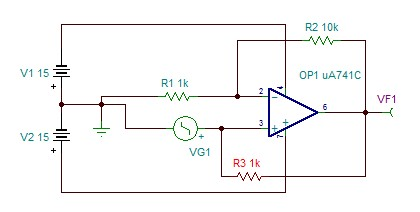
\includegraphics[scale=.6]{negatimpeconv}
\caption{Convertitore realizzato con TINA}
\label{fig:negimpcon}
\end{figure}

\begin{figure}[htp]
\centering
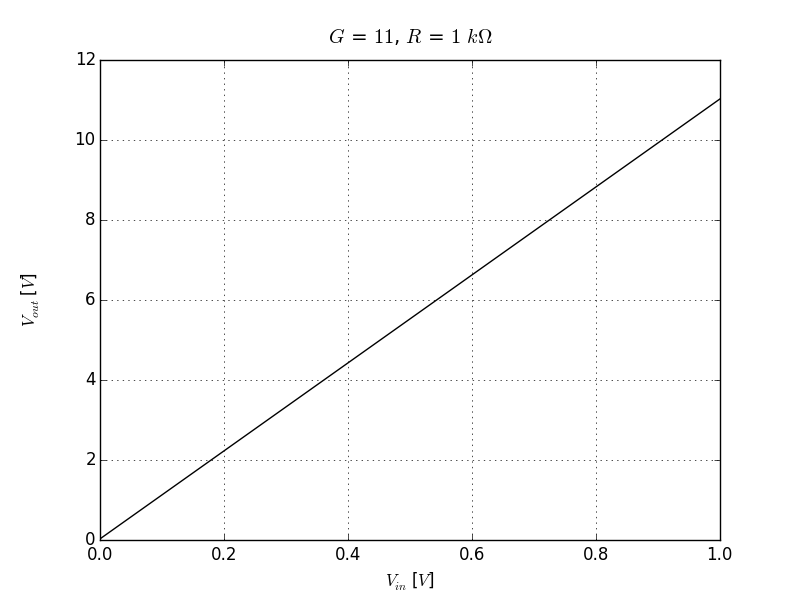
\includegraphics[scale=.35]{g_10_r_1k_dc_v}
\caption{Simulazione del convertitore per G=11}
\label{fig:g_10_r_1k_dc_v}
\end{figure}

\begin{figure}[htp]
\centering
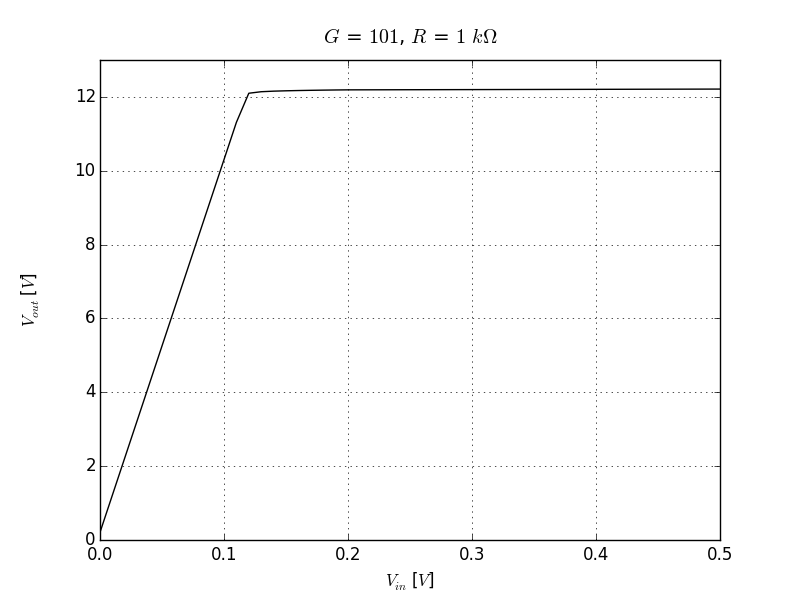
\includegraphics[scale=.35]{g_100_r_1k_dc_v}
\caption{Simulazione del convertitore con G=101}
\label{g_100_r_1k_dc_v}
\end{figure}

Per quanto riguarda $R_3$ invece, essa deve essere scelta in modo tale che non scorra troppa corrente verso il ramo non-invertente cosicché l'op-amp non riesca a stabilire il giusto feedback e dunque uguagliare le tensioni ai due ingressi, ovvero non deve essere troppo piccola. In figura \ref{g_10_r_300_dc_v} si vede come per tensioni vicine a 1 V si perda l'andamento lineare. 

\begin{figure}[htp]
\centering
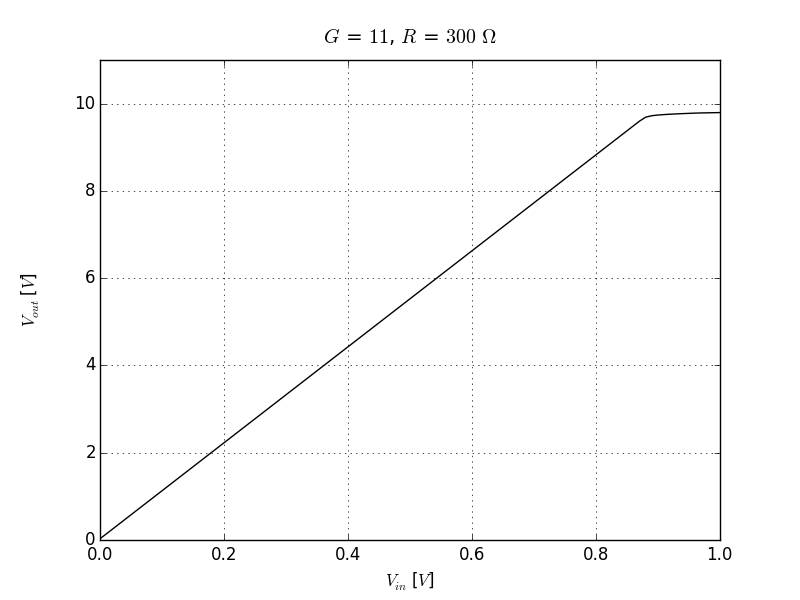
\includegraphics[scale=.35]{g_10_r_300_dc_v}
\caption{Simulazione del convertitore con G=11 e R=300 $\Omega$}
\label{g_10_r_300_dc_v}
\end{figure} 

Se si osserva il grafico in figura \ref{g_10_v_1_dc_r} si vede come per $V_{in} = 1 V$ il segnale in $V_{out}$ non dipenda da $R_3$ a partire dai 380 $\Omega$ circa.

\begin{figure}[htp]
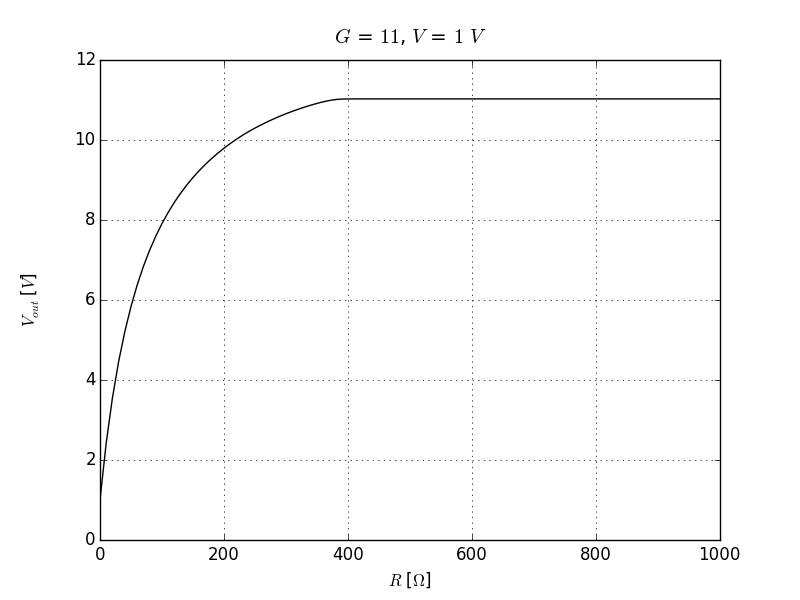
\includegraphics[scale=.4]{g_10_v_1_dc_r}
\caption{Dipendenza del segnale in uscita da $V_{out}$ in funzione di $R_3$ con G=11}
\label{g_10_v_1_dc_r} 
\end{figure}

Non disponendo di equazioni o modelli per dimensionare correttamente $R_3$, in base a varie prove effettuate possiamo fornire in tabella \ref{tab:r3} dei valori minimi indicativi per $R_3$ in funzione del gain G con una tensione di ingresso di 1 V.

\begin {table}[htp]
\caption {Valori minimi indicativi per $R_3$} 
\label{tab:r3} 
\begin{center}
\begin{tabular}{|c|c|}
\hline 
G & R \\ 
\hline 
11 & 380 \\ 
\hline 
10 & 230 \\ 
\hline 
9 & 150 \\ 
\hline 
8 & 110 \\ 
\hline 
7 & 80 \\ 
\hline 
6 & 60 \\ 
\hline 
\end{tabular} 
\end{center}
\end {table}

La possibilità di disporre di un circuito con impedenza equivalente negativa trova molte applicazioni, una di queste è il circuito di Howland.

\section{Circuito di Howland}

Lo schema del circuito di Howland è in figura \ref{fig:how}.

\begin{figure}[htp]
\centering
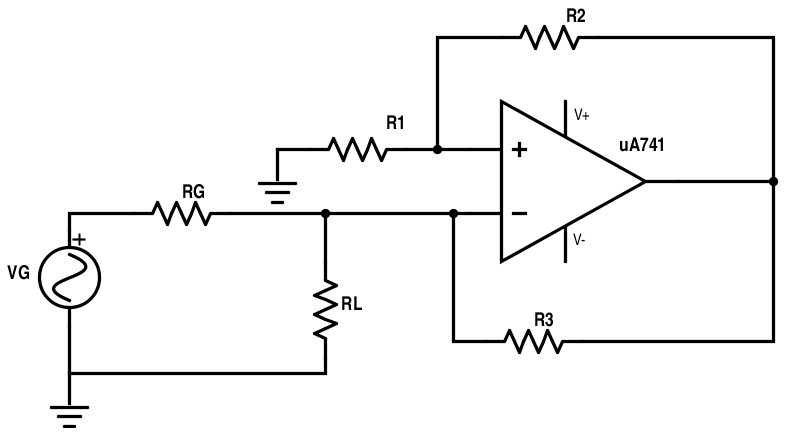
\includegraphics[scale=.3]{howland}
\caption{Circuito Howland}
\label{fig:how}
\end{figure}



\end{document}